\documentclass{beamer}
\usepackage{pdfpages}
\usepackage{graphicx}

% Remove navigation symbols
\setbeamertemplate{navigation symbols}{}

\title{Curse of Dimensionality}

\begin{document}

% \frame{\titlepage}

\begin{frame}{Overview}

\textbf{Source: } \url{https://slds-lmu.github.io/i2ml/chapters/14_cod/}

\begin{itemize}
    \item How our intuitions miserably fails as the dimensionality of the data increases
    \item Properties of high dimensional data
    \item Implications for distance based algorithms (e. g. KMeans, kNN)
    \item How to deal with those implications
    \item Most importantly - what happens if we peel a high dimensional mandarin (we will also have a practical session for the 3D case)
\end{itemize}
\end{frame}


\section{The Curse}
\includepdf[pages=2-18,scale=1.3,offset=50 -10]{slides-cod.pdf}

\section{ML Examples}
\includepdf[pages=2-last,scale=1.3,offset=50 -10]{slides-cod-examples.pdf}

\section{Pop Quiz}
\begin{frame}
    Why do we use cosine similarity instead of the Euclidean distance?
\end{frame}


\end{document}